\chapter{Implementation}

\section{Open Text Redaction Tool}
We introduce the \textbf{Open Text Redaction Tool (OpenTRT)} redaction method, an effective approach that strikes a balance between ensuring sufficient safety and maintaining accessibility. This method eliminates the to-be-redacted text from the visual content of the document by directly manipulating the PDF document. It allows for the replacement of the to-be-redacted text with a placeholder and manipulation of the positional adjustments for both redacted and non-redacted text. OpenTRT achieves effective redaction for PDF documents generated through the 'Save As PDF' functionality in Microsoft Word, specifically for documents originating in Word and not altered by any other software post-creation. While complete or partially effective redaction cannot be guaranteed for other workflows, it may still be attainable.
\\\\
Our tool/method is built upon the foundation of the \textit{PyMuPDF} \cite{PyMuPDF} Python library, a versatile tool for PDF manipulation and text redaction across various (PDF) documents. It offers support for extracting content and operations, removing and inserting text, as well as manipulating hidden information. To manipulate positional information and remove white spaces, we have devised a proprietary method for reading, interpreting, and manipulating content streams, building upon the functionality provided by PyMuPDF. Additionally, metadata manipulation is incorporated using the \textit{lxml.etree.ElementTree} library in conjunction with PyMuPDF.

\subsection{PyMuPDF}
Building upon the existing library has enabled us to support more documents, focus on the redaction and make the process easier. The library has certain flaws related to text selection and bounding boxes, and had no functionality to change positional information.  By addressing these issues and introducing functionality to modify positional information, we have successfully implemented redaction.


\section{Effective Text Redaction In Practice}
OpenTRT takes as input an unredacted PDF document created using the \textit{'Save As PDF'} functionality in Microsoft Word. This document should be originally crafted in Word and remain unaltered by any other software after creation. The input consists of machine-readable text within the PDF, not images of the document, along with a list of one or more character sequences and their corresponding bounding boxes per page. Each bounding box specifies the position of the text on a page. The list of character sequence bounding boxes should be ordered per page and position, following natural reading order (top-left to bottom-right).
\\\\
The output is a new PDF document where the specified character sequences have been effectively redacted from the document. Each redacted text element may have been replaced with an replacement value (defaulting to \textit{[x]}) and any non-redacted text may be repositioned to fill white spaces. 


\subsection{Algorithm}
The text redaction algorithm comprises four main steps, with optional steps in between. The process is illustrated using an example and pseudocode.

\subsubsection{0. PDF creation}
As an example, we begin with a randomly generated \textit{lorem ipsum} text pasted into a Word document. This document is then saved as a PDF, and the resulting file (see Appendix \ref{fig:example-pdf-lorem-ipsum}) serves as input for the algorithm.

\subsubsection{0.5. Redaction selection}
A redaction is 'selected' based on a bounding box which defines the position of a piece of text or character sequence on a page in a document. A bounding box can be defined as:

\[ (x0, y0, x1, y1). \]

Each redaction is also mapped to a specific page, ensuring that for every page, it is known which positions (bounding boxes) should be redacted.

\subsubsection{1. Text labelling and Selection}
Text is labelled based on the provided list of redactions. For each redaction, its corresponding bounding box is utilized as an argument in the \textit{get\_text()} method of PyMuPDF to extract the character sequence present in the bounding box. This returns the following:

\[((x0, y0, x1, y1), char\_seq, block\_no, line\_no, word\_no).\]

Each selected piece of text is defined by a rectangle, (x0, y0, x1, y1), another bounding box. When applying a redaction, an annotation is made with the exact dimension of the defined rectangle. Page content is then deleted based on intersection with a redaction annotation. With larger bounding boxes, it may occur that adjacent words or characters are unintentionally deleted. PyMuPDF natively defines a bounding box which tends to be bigger than the exact dimensions of the word. To address this, the redaction annotation is made smaller, ensuring that only the intended text is selected for redaction. 
\begin{lstlisting}[style=CStyle, caption=Pseudocode for labelling of text and the selection of the labels using PyMuPDF. Size of the bounding box is made smaller to prevent redaction of more than only the to-be-redacted text. This is an improvement of the original functionality of PyMuPDF which is prone to redacting more text than requested.]
# Get text of redactions
def select_redaction(redactions):

    redactions = []
    
    for redaction in redactions:
    
        # Get the text elements (words) within the specified bounding box (search result) and sort them in natural reading order
        text = page.get_text("words", clip=redaction bounding box, sort=True)
        
        redactions.add(text)

    return redactions

# Edit bounding boxes of redactions
def edit_bb(redactions):

    # Iterate through each redaction on the page
    for redaction in redactions on this page:
    
        # Get bounding box (rectangle) of redaction
        rect = redaction bounding box
    
        # Adjust the redact annotation to make it small
        
        # Height of the redaction rect
        h = rect height
        
        # Get new height of bounding box
        my = (rect.y0 + rect.y1) / 2 
        y0 = my - h * 0.1
        y1 = my + h * 0.1
        
        rect.y0 = y0
        rect.y1 = y1
    
        # Add the redaction to the page
        add_redaction(redaction, page)
\end{lstlisting}

\subsubsection{2. Removing text}
Once text has been located and its bounding box has been adjusted, all text intersecting with the rectangle of the redaction will be removed from the page. Removal occurs on a character basis; a character is eliminated if its bounding box has a non-empty overlap with the bounding box of the redaction. The removal of text is realised using the redaction functionality of PyMuPDF. Figure \ref{fig:redactannot1} shows text is selected for redaction using annotations which make use of the bounding box. After annotating all to-be-redacted text values, the \textit{apply\_redactions()} function removes any content contained within these redaction annotations, including any background color or other styling.

\begin{lstlisting}[style=CStyle, caption=Pseudocode for using the bounding boxes defined in the previous step as argument in the \textit{add\_redact\_annot()} PyMuPDF function and then applying them which removes any content from the selected area.]
# Add a single redaction annotation to a page
def add_redaction(redaction, page):
    page.add_redact_annot(redaction bounding box) # Add a redaction annotation to the file

# Apply redactions to a single page (no replacement value is inserted in the place)
def apply_redactions(page):
    page.apply_redactions()

\end{lstlisting}

\begin{figure}[h]
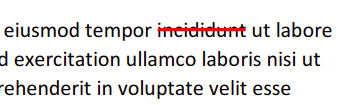
\includegraphics[width=0.5\textwidth]{latex/media/redactannot.png}
\centering
\caption{Before removing text, the to-be-removed text is highlighted using an redaction annotation from the PyMuPDF library. Because the bounding box has been made smaller in step 1, the actual annotation looks like a line which strikes through the text. Text is removed by PyMuPDF based on intersection and thus any content that intersects with the redaction annotation is removed from the document.}
\label{fig:redactannot1}
\end{figure}
\subsubsection{2.5 Replacement value}
A replacement text may be inserted, if desired, with the style (fontsize) based on the original character sequence. Replacement values are inserted onto a page using the original bounding box of the redacted value. Depending on the replacement value and the original text, the rectangle of the to-be-inserted text (initially the same as the original) may need adaptation to fit the new text. Leveraging the \textit{insert\_textbox()} function of PyMuPDF, which allows for text insertion onto a page using a bounding box, a replacement value is placed in the document. Figure \ref{fig:replacement} illustrates how replacements text can be used to indicate that text has been removed.

\begin{lstlisting}[style=CStyle, caption=Pseudocode for adding replacement text in place for the redacted text. The style of the replacement text is based on the original text. The bounding box which is used to insert the text in the document may be adapted to fit the text and position it correctly relative to other text.]
# For each redaction get some information for styling, determine the right bounding box to fit the new insertion value and finally insert it into the document.

for redaction in redactions on this page:
    fontsize = # based on the original redaction value
    font = a monospace font such as "Courier"

    # Determine length of replacement value "[x]" with fontsize=fontsize
    new_length = font.text_length("[x]", fontsize=fontsize)

    # Calculate the height needed for the text based on the font size
    new_height = (font.ascender - font.descender) * fontsize

    # Calculate the new x1 coordinate
    newx1 = rect[0] + new_length

    # Create a new rectangle for the text to be inserted
    new_rect = fitz.Rect(rect[0], rect[1], newx1, rect[1] + new_height)

    # Adapt the rect. based on the amount of space that is required
    While does_not_fit:
        # If not succesful return the space required to fit, else insert text
        space_too_much = page.insert_textbox(new_rect, "[x]", fontname=font_used, fontsize=fontsize)
        new_rect = # adapted based on the amount of space needed to fit the text

\end{lstlisting}

\begin{figure}[h]
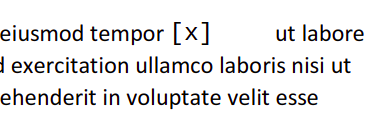
\includegraphics[width=0.5\textwidth]{latex/media/redactreplace.png}
\centering
\caption{After text removal, the to-be-redacted text has been removed and an optional replacement value has been inserted to visually indicate that some text has been redacted. The fontsize and position of the replacement value is based on the original redacted text. Depending on the length of the redacted character sequence, some white space or overlapping text may be present. In this case, the replacement value is shorter than the original value and thus some white space after the replacement value can be seen.}
\label{fig:replacement}
\end{figure}

\subsubsection{3. Manipulation of positional adjustments}
To adjust the positional information of text, all redactions and replacements must be mapped to the line on which they are present. This information is used to determine the content stream portion related to the line where a redaction was performed.
\\\\
Content streams may define text positions using the \textbf{Tm} operator 
(i.e. in Microsoft Word Schemes), which has four coordinate operands (x0, y0, x1, y1) specifying the bounding box of the text rendering operation. The left-lower point of this box is then calculated and compared to the y-coordinates of the redaction. If this point falls between or is equal to the y0 and y1 points of the redaction, it is considered part of the line. Additionally, it is checked if the candidate text element is part of the same text block as the redaction. 
\begin{lstlisting}[style=CStyle, caption=Pseudocode for identifying lines of text associated with each redaction based on their y-coordinates and text block.]
# For each redaction, find all associated operations in the content stream of a the page on which the redaction is.

# All operations of the content stream(s) of a page
for line in lines: 
    # Check if the line is a transformation matrix (ends with "Tm")
    if line.endswith("Tm") :
        x = x cord of Tm operation
        y = y cord of Tm operation

        # Create a rectangle representing the redaction
        rect = bounding box of redaction

        # Get the text block coordinates associated with the redaction
        block_cords = text block

        # Check if the current line is within the y-coordinates and text block coordinates
        if y >= redactions.y0 and y <= redaction.y3 and 
           y >= block.y0 and y <= block.y1 and 
           x >= block.x0 and x <= block.x1:

            # Iterate through subsequent lines until a TJ command is found
            for q in range(line, len(lines)):
                if lines[q].endswith("TJ"):
                    lines_per_line[redaction].add((lines[q], q, line)) # save operation, line number and Tm line
                    break

\end{lstlisting}
The sequence of commands extracted from the content stream is then parsed and the text rendering operations are then selected for further analysis. The textual content is separated from the positional information, which is manipulated based on its value. PyMuPDF adds a large horizontal shift (positional adjustment) after a redacted value to account for the space the original word took up. If a replacement value has been inserted, this positional adjustment is also modified to account for the length of this replacement value.
\\\\
If no replacement has been inserted, the adjustment is set to zero to eliminate any white space (figure \ref{fig:redactannot}). Depending on the text showing operator, this may result in words after the redaction also being shifted, achieving step 3.5 (section \ref{3.5}). Information associated with other text is rounded to a discrete value based on its initial value and a random factor between 0.2 and 1.8. This method increases the computational difficulty of determining the original positional adjustments and, consequently, the original redacted text. The following formula is used for the manipulation of the positional adjustments of non-redacted text:

\[newPositionalAdjustment = round(round(float(original\_value) * 0.0042 * randVal, 2) / 0.0042, 2),\]

\begin{lstlisting}[style=CStyle, caption=Pseudocode for manipulating possible positional adjustments based on value. A really big or really small value may be found which indicates that PyMuPDF has inserted a new value after redaction. A new positional adjustment is calculated based on the last redaction and replacement value. Other values are rounded to the nearest discrete value based on the initial value and a random factor.]
if value == "":
    # If no positional information, append an empty string as positional adjustment
    new_posadj.add("")
# Find re-positions
elif value > 100 or value < -100:
    if there are replacements on the line:
        l = width of last redaction
        m = width of last replacement
        b = (m / l)

        new_posadj.add(q * (b if b != 0 else 1.0))
    else:
        # If no replacements, 0 as new positonal adjustment
        new_posadj.add(0)
else:
    # Generate a random factor and calculate new positional adjustment
    rand = random.uniform(0.2, 1.8)
    
    newnum = formula to calculated rounded value
    
    new_posadj.add(newnum)
\end{lstlisting}

After manipulation, the text and its associated positional values are reassembled in the same order as extracted. This creates a new text rendering operation, replacing the old operation in the content stream. If there is no positional information in the text rendering operation, this step has no result.

\subsubsection{3.5 White space removal}
\label{3.5}
In documents where text is positioned using only Tm operations, textual content can be replaced by changing the operands associated with the Tm operations. Similar to positional adjustments, the first step is to determine which operations need adjustment, using the same method. For each of these text elements to be repositioned, the positional information is changed based on the difference between redacted and replacement text length. If no replacement value is present, only the redacted text length is considered. The updated operations are inserted back in the content stream, replacing the original operations.

\begin{figure}[h]
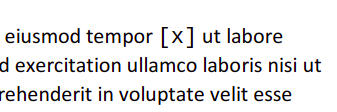
\includegraphics[width=0.5\textwidth]{latex/media/annotres.png}
\centering
\caption{Manipulation of positional information, either by changing positional adjustments in text rendering operations or text positioning operations, allows for the removal of spaces between words after redaction. Depending on the presence and length of replaced character sequence(s) and possible replacement value(s) text after the redaction is shifted to fill up white spaces resulting in neater document.}
\label{fig:redactannot}
\end{figure}
\subsubsection{4. Hidden information removal}
PyMuPDF automatically removes some of the hidden information which is associated with redacted text. Internal and external links are deleted from the document when the text containing the links is redacted. Any text covered by the to-be-redacted text is also removed. Furthermore, any unused attached and embedded files, content, invisible text, or any JavaScript can be optionally removed.
\\\\
For more intricate hidden information, such as (XML) metadata, manual examination is necessary as complete removal could potentially damage the accessibility of the document. Utilizing PyMuPDF and the \textit{lxml.etree.ElementTree} library, metadata content can be examined for possible character sequences that have been labelled. Each field in the metadata can be directly edited, simplifying the removal of any value through basic string manipulation.

\section{Limitations}
OpenTRT has limitations in terms of the types of PDF documents it supports due to complexity reasons. While the internal structure of PDF documents is generally consistent, the representation of content may vary significantly based on the method used to create the PDF. For example, text can be rendered in various ways with different combinations of operations, some more complex than others. Consequently, automating the process of effective redaction, including the manipulation of positional information, for a wide variety of documents becomes a challenging task. Given this complexity, we have restricted our focus to Microsoft Word and the way it represents text when saving a document as a PDF.
\\\\
Manipulating positional adjustments to enhance confidentiality can be achieved in multiple ways, as described in step \ref{posadj} of the effective redaction design. Having knowledge about the Microsoft Word schemes (the way Microsoft Word determines positional information) would have allowed for a more complex defense against deredaction of text. Unfortunately, while successful efforts have been made in reconstructing these schemes, this information appears to be somewhat confidential, and sharing it with other parties is not a viable option. A quick prototyping method, by directly editing documents in the docx format, may be an option, but it makes the process of reconstructing schemes even more complex and time-consuming. 
\\\\
Certain types of hidden information, such as attached and embedded files, are removed without examining their contents for any sensitive information. Files of different types could be associated with a PDF, and implementing comprehensive functionality to read and manipulate all of these would be beyond the scope of this project. Therefore, OpenTRT implements the removal of hidden information, excluding the (XML) metadata.
